\chapter{Grupy Pin i Spin, spinory oraz struktury spinowe}
\label{ch:lin31-spinory}

Algebrę Clifforda i jej reprezentację na algebrze zewnętrznej
zbudowaliśmy w Rozdziale~\ref{ch:lin30-clifford}.
W tym rozdziale przejdziemy od iloczynów wektorów jednostkowych
do grup Pin i Spin, a następnie do ich reprezentacji spinowych.
Ostatnia część dotyczy wiązek spinorowych nad rozmaitościami;
używamy w niej pojęć grassmannianu i wiązki wektorowej
wprowadzonych w Rozdziale~\ref{ch:lin29-grassmanniany}.

\section{Od odbić do grupy Spin}
\label{sec:lin31-spin-grupa}

Ustalmy najpierw dwie operacje na algebrze Clifforda.
Zmiana każdego $v$ na $-v$ zachowuje relacje definiujące,
więc daje automorfizm $\alpha$, z $\alpha^2=\id$.
Jego przestrzenie własne dla $+1$ i $-1$ są rozpięte
odpowiednio przez słowa parzyste i nieparzyste; dowód bazy
pokazuje, że ich suma jest prosta.
Drugą operacją jest \emph{rewersja}, oznaczana tyldą:
\[
 \widetilde{v_1\cdots v_r}=v_r\cdots v_1,\qquad
 \widetilde 1=1,
\]
przedłużona liniowo. Jest dobrze określona na ilorazie:
odwracanie słów w $T(V)$ ustala każdy generator
$v\otimes v+\|v\|^2 1$, a element $a(v\otimes v+\|v\|^2 1)b$
wysyła na $\widetilde b(v\otimes v+\|v\|^2 1)\widetilde a$,
nadal należący do ideału. Zatem
$\widetilde{st}=\widetilde t\,\widetilde s$ i
$\widetilde{\widetilde s}=s$, niezależnie od zapisu $s$ jako sumy słów.

Odbicie względem hiperpłaszczyzny prostopadłej
do jednostkowego $u\in V$ ma wzór
\begin{equation}\label{eq:lin31-spin-odbicie}
 r_u(v)=v-2\langle u,v\rangle u.
\end{equation}
Rozkład $v=\langle u,v\rangle u+w$, $w\perp u$,
pokazuje, że $r_u$ odwraca składową równoległą do $u$
i zostawia składową $w$. Jego wyznacznik jest równy $-1$.
Relacja Clifforda daje zaskakujący opis tego odbicia:
ponieważ $u^2=-1$, mamy $u^{-1}=-u$ i
\[
 -uvu^{-1}=uvu
 =-vu^2-2\langle u,v\rangle u
 =v-2\langle u,v\rangle u
 =r_u(v).
\]
W środkowej równości użyliśmy
$uv=-vu-2\langle u,v\rangle$. Znak minus przed
sprzężeniem jest niezbędny, aby obrazem było odbicie
w hiperpłaszczyźnie $u^\perp$ w każdym wymiarze.
Na przykład w $\R^3$ dla $u=e_1$ zwykłe sprzężenie
$v\mapsto uvu^{-1}$ ma w bazie standardowej macierz
$\operatorname{diag}(1,-1,-1)$, natomiast skręcone sprzężenie
$v\mapsto-uvu^{-1}$ ma macierz $\operatorname{diag}(-1,1,1)$.

\begin{definicja}[Grupa Pin]
\label{def:lin31-pin-grupa}
\index{grupa pin@Grupa Pin}
Dla euklidesowej przestrzeni $V$ grupą $\operatorname{Pin}(V)$
nazywamy podgrupę odwracalnych elementów $\operatorname{Cl}(V)$
złożoną ze wszystkich skończonych iloczynów wektorów
jednostkowych; dopuszczamy pusty iloczyn $1$.
W odróżnieniu od grupy Spin dopuszczamy także nieparzystą
liczbę czynników. Dla $s\in\operatorname{Pin}(V)$ określamy
\[
 \rho_{\mathrm{Pin}}(s)(v):=\alpha(s)v s^{-1},
 \qquad v\in V,
\]
gdzie $\alpha$ zmienia znak każdego wektora, jak wyżej.
\end{definicja}

Wzór jest skręconym sprzężeniem: dla jednostkowego $u$
daje $\rho_{\mathrm{Pin}}(u)(v)=-uvu^{-1}=r_u(v)$.
Zatem pojedynczy wektor reprezentuje odbicie, a jego parzysty
iloczyn reprezentuje obrót. Na przykład w $\R^2$ element
$e_1\in\operatorname{Pin}(2)$ daje odbicie w prostej
$e_1^\perp$: wysyła $e_1$ na $-e_1$, a $e_2$ pozostawia
bez zmiany. Z kolei $e_1e_2$ daje złożenie odbić
$r_{e_1}r_{e_2}=-\id_{\R^2}$, czyli obrót o pół obiegu.
Przy przyjętej relacji $u^2=-\|u\|^2$ grupa ta bywa
oznaczana $\operatorname{Pin}^{-}(n)$; znak rozróżnia dwie
konwencje algebry Clifforda.

\begin{definicja}[Grupa Spin]
\index{grupa spin@Grupa Spin}
\label{def:lin31-spin-grupa}
Niech $n=\dim V\geq2$. \emph{Grupą spinową}
$\operatorname{Spin}(V)$ nazywamy podgrupę
odwracalnych elementów $\operatorname{Cl}(V)$,
składającą się z iloczynów \emph{parzystej}
liczby wektorów jednostkowych:
\[
 \operatorname{Spin}(V)
 :=\{u_1\cdots u_{2r}:\|u_j\|=1,\ r\geq0\}.
\]
Pusty iloczyn to $1$. Skrót
$\operatorname{Spin}(n)$ oznacza
$\operatorname{Spin}(\R^n)$ ze standardową metryką.
Dla $s\in\operatorname{Spin}(V)$ określamy
$\rho(s)v:=svs^{-1}$.
Topologię na grupie bierzemy z jej inkluzji do skończenie
wymiarowej przestrzeni $\operatorname{Cl}(V)$. Gładką strukturę
zgodną z tą inkluzją uzasadnimy w dowodzie nakrycia.
\end{definicja}

Zbiór w definicji jest grupą: iloczyn dwóch słów
parzystych jest parzysty, a odwrotność słowa
$u_1\cdots u_{2r}$ to
$(-u_{2r})\cdots(-u_1)$, ponownie słowo parzyste
złożone z wektorów jednostkowych.
Każdy jego czynnik ma dobrze określoną odwrotność.

\begin{twierdzenie}[Dwukrotne nakrycie grupy obrotów]
\label{thm:lin31-spin-nakrycie}
Przypisanie $\rho$ jest surjektywnym homomorfizmem
\[
 \rho:\operatorname{Spin}(n)\longrightarrow\mathrm{SO}(n),
 \qquad\ker\rho=\{1,-1\}.
\]
Jest gładkim dwukrotnym nakryciem: każdy obrót
ma dokładnie dwa podniesienia $s$ i $-s$.
\end{twierdzenie}
\begin{proof}
\emph{Dlaczego obrazem jest obrót?}
Dla słowa $s=u_1\cdots u_{2r}$ zastosujmy
wzór na odbicie do kolejnych czynników.
W odwzorowaniu $v\mapsto-u v u^{-1}$ pojawia się
jedno odbicie $r_u$; przy parzystej liczbie
czynników wszystkie minusy się znoszą i
\[
 \rho(s)=r_{u_1}\circ\cdots\circ r_{u_{2r}}.
\]
To złożenie zachowuje iloczyn skalarny i ma
wyznacznik $(-1)^{2r}=1$. Ponieważ
$\rho(st)(v)=s(tvt^{-1})s^{-1}$,
$\rho$ jest homomorfizmem do $\mathrm{SO}(n)$.

\emph{Dlaczego jest surjektywna?}
Pokażmy elementarnie, że każdą izometrię liniową
można zapisać jako iloczyn odbić. Weźmy bazę
ortonormalną $e_1,\ldots,e_n$ i $A\in\mathrm O(n)$.
Jeśli $Ae_1\ne e_1$, to dla
$u=(Ae_1-e_1)/\|Ae_1-e_1\|$ rachunek z
\eqref{eq:lin31-spin-odbicie} daje $r_u(Ae_1)=e_1$:
licznik iloczynu
$\langle Ae_1-e_1,Ae_1\rangle$ to
$1-\langle Ae_1,e_1\rangle$, a kwadrat
mianownika to $2(1-\langle Ae_1,e_1\rangle)$.
Jeśli $Ae_1=e_1$, pomijamy ten krok.
Nowa izometria zachowuje $e_1$, więc działa
na $e_1^\perp$. Powtarzamy argument dla $e_2$
w tym dopełnieniu, potem dla $e_3$, itd.
Po skończenie wielu krokach otrzymujemy
identyczność. Zapisujemy więc $A$ jako
iloczyn odbić. Ponieważ $\det A=1$, liczba
użytych odbić musi być parzysta; odpowiadający
im iloczyn jednostkowych $u_j$ jest szukanym
elementem $\operatorname{Spin}(n)$.

\emph{Dlaczego jądro ma tylko dwa elementy?}
Niech $s$ działa trywialnie na $V$. Wtedy
$se_j=e_js$ dla każdego wektora bazy ortonormalnej.
Rozwińmy $s$ w bazie z
Twierdzenia~\ref{thm:lin30-cliff-baza}, używając tylko
słów parzystej długości:
$s=\sum_{|I|\ {\rm parzyste}}a_I e_I$.
Dla parzystego niepustego $I$ i $j\in I$
relacja~\eqref{eq:lin30-cliff-orto} daje
$e_je_Ie_j^{-1}=-e_I$; gdy $j\notin I$,
otrzymujemy $+e_I$.
Rzeczywiście, jeśli $j\notin I$, przenosimy $e_j$
przez $|I|$ różnych generatorów i dostajemy znak
$(-1)^{|I|}=1$. Jeśli $j\in I$, mija on tylko
$|I|-1$ innych generatorów, co daje znak $-1$;
czynnik $e_je_j^{-1}$ następnie się skraca. Równość
$e_jse_j^{-1}=s$ dla \emph{wszystkich} $j$
wymusza więc $a_I=0$ dla każdego niepustego $I$.
Zatem $s=a\,1$. Aby ustalić $a$, odwróćmy
porządek wektorów w słowie:
$\widetilde s=u_{2r}\cdots u_1$.
Wtedy $s\widetilde s=(-1)^{2r}=1$,
bo wektory są jednostkowe i $u_i^2=-1$.
Dla skalarnego $s=a$ również $\widetilde s=a$,
stąd $a^2=1$. Oba znaki występują,
gdyż $-1=e_1e_1\in\operatorname{Spin}(n)$.

\emph{Dlaczego rzeczywiście jest to nakrycie?}
Grupa $\mathrm O(n)$ jest gładką podrozmaitością
przestrzeni rzeczywistych macierzy. Aby to uzasadnić,
rozważmy odwzorowanie $F(A)=A^TA-I$ o wartościach w
przestrzeni macierzy symetrycznych. W punkcie ortogonalnym
$Q$ jego różniczka to
$DF_Q(H)=Q^TH+H^TQ$. Dla dowolnej macierzy symetrycznej
$S$ wybór $H=\frac12 QS$ daje $DF_Q(H)=S$,
więc różniczka jest surjektywna. Z twierdzenia o funkcji
uwikłanej wynika, że $F^{-1}(0)=\mathrm O(n)$
jest gładką podrozmaitością o wymiarze $n(n-1)/2$.
Warunek $\det A=1$ wycina w niej otwartą i domkniętą
podrozmaitość $\mathrm{SO}(n)$.
Pokażmy, że w pobliżu identyczności obroty mają
gładko wybrane podniesienie. Dla bliskich
jednostkowych $a,b$ połóżmy
\[
 R(a,b):=-\frac{a+b}{\|a+b\|}\,a
       =\frac{1-ba}{\|a+b\|}\in\operatorname{Spin}(n).
\]
Jest to iloczyn dwóch jednostkowych wektorów,
zależy gładko od $(a,b)$, spełnia $R(a,a)=1$
i przenosi $a$ na $b$: pierwsze odbicie w
hiperpłaszczyźnie do $a$ wysyła $a$ na $-a$,
drugie, o normalnej $(a+b)/\|a+b\|$, wysyła
$-a$ na $b$.
W tym ostatnim kroku $u=(a+b)/\|a+b\|$ i wzór na odbicie dają
\[
 r_u(-a)
 =-a+\frac{2(1+\langle a,b\rangle)}{\|a+b\|^2}(a+b)
 =-a+(a+b)=b,
\]
ponieważ $\|a+b\|^2=2(1+\langle a,b\rangle)>0$.
Jeśli $A$ jest bliski identyczności,
stosujemy taki rotor, aby skorygować $Ae_1$ do
$e_1$. Otrzymany obrót zachowuje $e_1$.
W $e_1^\perp$ korygujemy następnie obraz
$e_2$, potem $e_3$, kończąc na $e_{n-1}$;
ostatni wektor jest ustalony dzięki wyznacznikowi
$1$. Każdy rotor zależy gładko od $A$
w niewielkim otoczeniu identyczności.
Odwrotność ich iloczynu daje gładką lokalną
sekcję $\sigma$ odwzorowania $\rho$.
Przy innym obrocie przenosimy to otoczenie
przez ustalony element z jego przeciwobrazu.
Wybierzmy otoczenie $U$ identyczności w $\mathrm{SO}(n)$
tak małe, aby $\sigma(A)$ było określone i współczynnik
przy $1$ w jego rozwinięciu w bazie Clifforda był większy
niż $1/2$ dla każdego $A\in U$; jest to możliwe, bo
$\sigma(\id)=1$. Obliczone jądro daje dokładnie
\[
 \rho^{-1}(U)=\sigma(U)\sqcup(-\sigma(U)).
\]
Pierwszy zbiór jest przecięciem $\rho^{-1}(U)$
z otwartym warunkiem dodatniości współczynnika skalarnego,
drugi odpowiada warunkowi ujemności tego współczynnika.
Oba są więc otwarte w $\operatorname{Spin}(n)$, a $\rho$
odwzorowuje każdy z nich homeomorficznie na $U$:
odwrotnościami są ciągłe odwzorowania $\sigma$ i $-\sigma$.
Mnożenie przez ustalone podniesienie przenosi tę konstrukcję
nad otoczenie dowolnego obrotu. Otrzymaliśmy zatem
dwukrotne nakrycie.
W ten sposób otrzymujemy także atlas gładki: na każdym płacie
używamy współrzędnych z $\mathrm{SO}(n)$ przeniesionych przez $\rho$.
Jest on zgodny z inkluzją do algebry Clifforda. Istotnie,
$\sigma$ jest gładka jako odwzorowanie do tej algebry, a pochodna
$\rho\circ\sigma=\id$ jest identycznością. Do różniczkowania
$\rho$ w otoczeniu płata wystarczy gładki wzór
$s\mapsto(v\mapsto\operatorname{pr}_V(svs^{-1}))$
na otwartym zbiorze elementów odwracalnych; na grupie Spin
rzut $\operatorname{pr}_V$ na składnik $V$ w bazie
z Twierdzenia~\ref{thm:lin30-cliff-baza} niczego nie zmienia.
Wynika stąd iniektywność różniczki $\sigma$; ponieważ
$\rho|_{\sigma(U)}$ jest odwrotnością $\sigma$, płat
jest lokalnie podrozmaitością algebry Clifforda. Mnożenie jest
dwuliniowe, a odwracanie gładkie: można je obliczać przez
odwracanie macierzy lewego mnożenia. Obie operacje ograniczają
się więc do gładkich operacji grupy Spin, a $\rho$ jest lokalnym dyfeomorfizmem.
\end{proof}

\begin{wniosek}[Nakrycie grupy ortogonalnej przez Pin]
\label{cor:lin31-pin-nakrycie}
Dla $n\geq2$ odwzorowanie
\[
 \rho_{\mathrm{Pin}}:\operatorname{Pin}(n)\longrightarrow
 \mathrm O(n)
\]
jest surjektywnym homomorfizmem o jądrze $\{1,-1\}$.
Jest gładkim dwukrotnym nakryciem, a przeciwobraz
$\mathrm{SO}(n)$ jest równy $\operatorname{Spin}(n)$.
\end{wniosek}
\begin{proof}
Automorfizm $\alpha$ jest multiplikatywny, więc
$\rho_{\mathrm{Pin}}(st)=\rho_{\mathrm{Pin}}(s)
\rho_{\mathrm{Pin}}(t)$. Każdy czynnik jednostkowy
daje odbicie. Rozkład izometrii na odbicia wykonano
w dowodzie Twierdzenia~\ref{thm:lin31-spin-nakrycie}; zapewnia
on surjektywność. Wyznacznik obrazu iloczynu $r$
wektorów wynosi $(-1)^r$. Parzyste słowa tworzą
zatem dokładnie przeciwobraz $\mathrm{SO}(n)$, czyli
$\operatorname{Spin}(n)$. Element jądra musi być parzysty,
a jądro na $\operatorname{Spin}(n)$ obliczono w tym samym
twierdzeniu jako $\{\pm1\}$. Lokalnie nad składową
$\mathrm{SO}(n)$ mamy już dwa gładkie płaty nakrycia Spin.
Mnożenie przez ustalony wektor jednostkowy przenosi je
na drugą składową $\mathrm O(n)$, co dowodzi ostatniej tezy.
\end{proof}

\begin{przyklad}[Dlaczego pojawia się połowa kąta?]
\label{prz:lin31-spin2}
W płaszczyźnie $B=e_1e_2$ spełnia $B^2=-1$.
Ponieważ część parzysta ma bazę $(1,B)$,
jej elementy mają postać $a+bB$. Dla słów
należących do $\operatorname{Spin}(2)$ równość
$s\widetilde s=1$ z poprzedniego dowodu daje
$a^2+b^2=1$. Odwrotnie, jeśli
$a=\cos t$, $b=\sin t$, to
\[
 a+bB=(-\cos t\,e_1-\sin t\,e_2)e_1,
\]
czyli iloczyn dwóch jednostkowych wektorów.
Grupa $\operatorname{Spin}(2)$ jest zatem okręgiem.
Połóżmy
\[
 s_\theta=\cos(\theta/2)+\sin(\theta/2)B.
\]
Korzystając z $Be_1=e_2$ i $Be_2=-e_1$,
oznaczmy $c=\cos(\theta/2)$ i $d=\sin(\theta/2)$.
Ponieważ $B^2=-1$, mamy $s_\theta^{-1}=c-dB$.
Obliczamy kolejno
\[
 s_\theta e_1s_\theta^{-1}
 =(ce_1+de_2)(c-dB)
 =(c^2-d^2)e_1+2cd\,e_2
 =\cos\theta\,e_1+\sin\theta\,e_2.
\]
Dla drugiego wektora $Be_2=-e_1$ daje
$s_\theta e_2s_\theta^{-1}
=(ce_2-de_1)(c-dB)
=-2cd\,e_1+(c^2-d^2)e_2
=-\sin\theta\,e_1+\cos\theta\,e_2$.
Jeden pełny obrót ma zatem podniesienie
$s_{2\pi}=-1$, a dopiero $s_{4\pi}=1$.
Po utożsamieniu obu grup z okręgiem odwzorowanie
$\rho$ ma postać $z\mapsto z^2$.
\end{przyklad}

\begin{figure}[!htbp]
\centering
\begin{tikzpicture}[>=Stealth,line cap=round]
 \draw[manifoldblue!75!black,thick] (-2.45,0) circle (1.03);
 \draw[manifoldgreen!75!black,thick] (2.45,0) circle (1.03);
 \draw[manifoldred,very thick,postaction={decorate},
  decoration={markings,mark=at position .55 with {\arrow{Stealth}}}]
  (-1.42,0) arc[start angle=0,end angle=180,radius=1.03];
 \draw[manifoldgreen!75!black,very thick,postaction={decorate},
  decoration={markings,mark=at position .78 with {\arrow{Stealth}}}]
  (3.48,0) arc[start angle=0,end angle=360,radius=1.03];
 \fill[manifoldblue] (-1.42,0) circle (2.2pt)
  node[right,font=\small] {$1$};
 \fill[manifoldred] (-3.48,0) circle (2.2pt)
  node[left,font=\small] {$-1$};
 \fill[manifoldgreen!70!black] (3.48,0) circle (2.2pt)
  node[right,font=\small] {$\id$};
 \draw[->,thick,manifoldgold!85!black] (-.84,0)--(.84,0)
  node[midway,above,font=\small] {$\rho:z\mapsto z^2$};
 \node[font=\small,manifoldblue!75!black] at (-2.45,-1.52)
  {$\operatorname{Spin}(2)$: pół obiegu};
 \node[font=\small,manifoldgreen!70!black] at (2.45,-1.52)
  {$\mathrm{SO}(2)$: cały obrót};
\end{tikzpicture}
\caption{Droga od $1$ do $-1$ w $\operatorname{Spin}(2)$
rzutuje się na pełen obrót w $\mathrm{SO}(2)$.
Końce drogi są różne w grupie Spin, choć odpowiadają
temu samemu obrotowi.}
\label{fig:lin31-spin-dwukrotne}
\end{figure}

\begin{przyklad}[Trzy wymiary: kwaterniony]
\label{prz:lin31-spin3}
W $\operatorname{Cl}(\R^3)$ część parzysta ma bazę
$1,I=e_2e_3,J=e_3e_1,K=e_1e_2$.
Na przykład z \eqref{eq:lin30-cliff-orto}
$I^2=e_2e_3e_2e_3=-e_2^2e_3^2=-1$ oraz
$IJ=e_2e_3e_3e_1=-e_2e_1=e_1e_2=K$.
Cykliczna zamiana indeksów $1,2,3$ daje
$J^2=K^2=-1$, $JK=I$ i $KI=J$.
Iloczyny w odwrotnej kolejności mają przeciwne znaki;
na przykład $JI=e_3e_1e_2e_3=-e_1e_2=-K$.
Jest to algebra kwaternionów $\mathbb H$.
Odwracanie kolejności czynników wysyła
$a+bI+cJ+dK$ na $a-bI-cJ-dK$,
więc $s\widetilde s=a^2+b^2+c^2+d^2$.
Istotnie, dla $q=bI+cJ+dK$ mieszane składniki $q^2$
znikają, bo $IJ+JI=JK+KJ=KI+IK=0$.
Stąd $q^2=-(b^2+c^2+d^2)$ i
$(a+q)(a-q)=a^2-q^2$ daje tę równość.
Każdy element $\operatorname{Spin}(3)$
jest zatem jednostkowym kwaternionem.
I odwrotnie, dowolny jednostkowy kwaternion
można zapisać jako $\cos t+\sin t\,B$,
gdzie $B$ jest jednostkowym dwuwektorem
w $\R^3$ (przypadki $\pm1$ są natychmiastowe).
Każdy taki $B$ jest iloczynem dwóch
prostopadłych wektorów jednostkowych. Aby to sprawdzić,
zapiszmy $B=b e_2e_3+c e_3e_1+d e_1e_2$ z $b^2+c^2+d^2=1$.
Wybierzmy jednostkowy $u\perp n=(b,c,d)$ i połóżmy
$v=n\times u$. Wtedy $u,v$ są ortonormalne i $u\times v=n$.
Współczynniki $u\wedge v$ w bazie
$(e_2\wedge e_3,e_3\wedge e_1,e_1\wedge e_2)$ są właśnie $(b,c,d)$,
więc $uv=B$. Z kolei
$\cos t+\sin t\,B$ jest także iloczynem dwóch
wektorów jednostkowych: jeśli $B=uv$ dla
$u\perp v$, to wprost z $vu=-uv$ i $u^2=-1$
otrzymujemy
\[
 (-\cos t\,u-\sin t\,v)u
     =\cos t+\sin t\,uv.
\]
Zatem $\operatorname{Spin}(3)\cong S^3$
jako grupa jednostkowych kwaternionów,
a $\rho:S^3\to\mathrm{SO}(3)$ utożsamia
parę $s,-s$.
\end{przyklad}

\section{Spinory: moduły algebry Clifforda}
\label{sec:lin31-spinory}

Wektor w $\R^n$ obraca się przez $\rho(s)\in\mathrm{SO}(n)$.
Spinor ma podlegać działaniu samego $s\in\operatorname{Spin}(n)$,
tak aby dwa podniesienia tego samego obrotu mogły
działać odmiennie. Do opisania wszystkich wymiarów
użyjemy liczb zespolonych. \emph{Zespolenie}
$\operatorname{Cl}^{\C}_n:=
\operatorname{Cl}(\R^n)\otimes_\R\C$
ma tę samą bazę uporządkowanych słów co algebra
rzeczywista, ale współczynniki zespolone.
Jego wymiar nad $\C$ wynosi $2^n$.

\begin{definicja}[Spinor zespolony]
\index{spinor zespolony@Spinor zespolony}
\label{def:lin31-spinor}
\emph{Moduł} algebry $A$ nad $\mathbb K$ to przestrzeń liniowa
$\Delta$ nad $\mathbb K$ z działaniem $A\times\Delta\to\Delta$
dwuliniowym nad $\mathbb K$ i zgodnym
z mnożeniem: $(ab)\psi=a(b\psi)$
oraz $1\psi=\psi$. Jest \emph{nieredukowalny},
jeśli $\Delta\ne0$ i nie ma właściwej niezerowej podprzestrzeni
zachowywanej przez wszystkie działania $a\in A$.
W tym rozdziale \emph{przestrzenią spinorów}
w wymiarze $n$ nazwiemy nieredukowalny zespolony
moduł $\Delta_n$ algebry $\operatorname{Cl}^{\C}_n$.
Jej element $\psi$ to spinor. Ograniczenie
działania do $\operatorname{Spin}(n)\subset
\operatorname{Cl}^{\C}_n$ jest
\emph{reprezentacją spinową}.
\end{definicja}

Słowo \emph{moduł} brzmi abstrakcyjnie, lecz tutaj
oznacza po prostu konkretne macierze $c(v)$
działające na kolumny $\psi$, z warunkiem
$c(v)^2=-\|v\|^2 I$. Działanie na całej algebrze
jest wtedy wyznaczone przez jej własność uniwersalną.
Przykładem modułu jest $\Lambda V$ z dowodu
Twierdzenia~\ref{thm:lin30-cliff-baza}, ale zwykle jest
on \emph{większy} niż nieredukowalna przestrzeń
spinorów. Nie należy więc utożsamiać automatycznie
wielowektora ze spinorem.

\begin{przyklad}[Macierze Pauliego]
\label{prz:lin31-pauli}
Niech
\[
 \sigma_1=\begin{pmatrix}0&1\\1&0\end{pmatrix},
 \quad
 \sigma_2=\begin{pmatrix}0&-i\\i&0\end{pmatrix},
 \quad
 \sigma_3=\begin{pmatrix}1&0\\0&-1\end{pmatrix}.
\]
Kwadraty $\sigma_1,\sigma_3$ są identycznością,
a dla $\sigma_2$ dwa diagonalne współczynniki kwadratu
to $(-i)i=i(-i)=1$, przy zerowych pozostałych.
Trzy niezależne iloczyny różnych macierzy wynoszą
\[
 \begin{aligned}
 \sigma_1\sigma_2&=\begin{pmatrix}i&0\\0&-i\end{pmatrix}
                  =i\sigma_3,\\
 \sigma_2\sigma_3&=\begin{pmatrix}0&i\\i&0\end{pmatrix}
                  =i\sigma_1,\\
 \sigma_3\sigma_1&=\begin{pmatrix}0&1\\-1&0\end{pmatrix}
                  =i\sigma_2.
 \end{aligned}
\]
Każda $\sigma_j$ jest hermitowska.
Sprzężenie tych trzech równości daje więc iloczyny w odwrotnej
kolejności: $(\sigma_i\sigma_j)^*=\sigma_j\sigma_i$,
a $(i\sigma_k)^*=-i\sigma_k$.
Otrzymaliśmy $\sigma_i^2=I_2$ oraz
$\sigma_i\sigma_j=-\sigma_j\sigma_i$ dla $i\ne j$.
Macierze $c(e_j)=i\sigma_j$ spełniają więc
\[
 c(e_i)c(e_j)+c(e_j)c(e_i)=-2\delta_{ij}I_2.
\]
Dla $n=2$ wystarczą $c(e_1),c(e_2)$.
Ich iloczyn to $-i\sigma_3$, a cztery macierze
$I_2,i\sigma_1,i\sigma_2,-i\sigma_3$
są liniowo niezależne i rozpinają
$M_2(\C)$. Aby sprawdzić niezależność, przyrównujemy
ich kombinację do macierzy zerowej:
\[
 \alpha I_2+\beta i\sigma_1+\gamma i\sigma_2-\delta i\sigma_3
 =\begin{pmatrix}
   \alpha-i\delta&i\beta+\gamma\\
   i\beta-\gamma&\alpha+i\delta
  \end{pmatrix}=0.
\]
Dodanie i odjęcie równań diagonalnych daje
$\alpha=\delta=0$, a pozostałych $\beta=\gamma=0$.
W przestrzeni wymiaru $4$ te cztery macierze tworzą więc bazę.
Z wymiaru $4$ obu stron dostajemy
$\operatorname{Cl}^{\C}_2\cong M_2(\C)$.
Przestrzeń spinorów $\Delta_2=\C^2$
jest zwykłą przestrzenią kolumn długości $2$.
\end{przyklad}

\begin{twierdzenie}[Klasyfikacja zespolona i wymiar spinorów]
\label{thm:lin31-cliff-kompleks}
Dla $m\geq0$ istnieją izomorfizmy algebr
\begin{align}
 \operatorname{Cl}^{\C}_{2m}
   &\cong M_{2^m}(\C), \label{eq:lin31-cliff-complex-even}\\
 \operatorname{Cl}^{\C}_{2m+1}
   &\cong M_{2^m}(\C)\oplus M_{2^m}(\C).
   \label{eq:lin31-cliff-complex-odd}
\end{align}
Wobec tego nieredukowalny moduł zespolony
ma wymiar $2^{\lfloor n/2\rfloor}$.
Dla parzystego $n$ jest jeden taki moduł
z dokładnością do izomorfizmu, a dla
nieparzystego $n$ są dwa.
\end{twierdzenie}
\begin{proof}
W wymiarze $0$ algebra ma postać $\C$.
W wymiarze $1$ składa się z $a+be_1$ przy
$e_1^2=-1$. Homomorfizm
$a+be_1\mapsto(a+bi,a-bi)$ powstaje przez podstawienia
$e_1=i$ i $e_1=-i$.
Ma odwrotność
$(z_+,z_-)\mapsto(z_++z_-)/2+(z_+-z_-)\,e_1/(2i)$,
więc daje $\operatorname{Cl}^{\C}_1\cong\C\oplus\C$.
Przykład~\ref{prz:lin31-pauli} daje
$\operatorname{Cl}^{\C}_2\cong M_2(\C)$.

Wykażmy krok indukcyjny zwiększający wymiar o $2$.
Iloczyn tensorowy algebr wyposażamy tu w mnożenie
$(a\otimes A)(b\otimes B)=ab\otimes AB$, rozszerzone
dwuliniowo; własność uniwersalna iloczynu tensorowego zapewnia
jego poprawne określenie. Łączność sprawdzamy na tensorach
prostych, a jedynką jest $1\otimes I_2$.
Niech $e_1,\ldots,e_n$ będą generatorami
$\operatorname{Cl}^{\C}_n$. W algebrze
$\operatorname{Cl}^{\C}_n\otimes M_2(\C)$
weźmy $n+2$ elementów:
\[
 F_j=e_j\otimes\sigma_3\ (j\leq n),\qquad
 F_{n+1}=1\otimes i\sigma_1,\qquad
 F_{n+2}=1\otimes i\sigma_2.
\]
Każdy $F_j^2=-1$. Dwa różne elementy
antykomutują: dla $j,\ell\leq n$ wynika
to z relacji starych $e_j$; między pierwszymi
$n$ a ostatnimi dwoma wynika z tego, że
$\sigma_3$ antykomutuje z $\sigma_1,\sigma_2$;
ostatnie dwa antykomutują jako macierze Pauliego.
Własność uniwersalna daje homomorfizm
\[
 \operatorname{Cl}^{\C}_{n+2}
    \longrightarrow
   \operatorname{Cl}^{\C}_n\otimes M_2(\C).
\]
Obrazy dwóch ostatnich generatorów dają całą
podalgebrę $1\otimes M_2(\C)$:
ich iloczyn jest $-i(1\otimes\sigma_3)$,
a wraz z jedynką tworzą bazę czterech macierzy.
Następnie z
$(e_j\otimes\sigma_3)(1\otimes\sigma_3)
=e_j\otimes I_2$ otrzymujemy wszystkie
generatory pierwszego czynnika. Homomorfizm
jest więc surjektywny. Obie algebry mają
wymiar $2^{n+2}$ nad $\C$
(Twierdzenie~\ref{thm:lin30-cliff-baza}),
więc jest izomorfizmem. Używamy przy tym
$M_d(\C)\otimes M_2(\C)\cong M_{2d}(\C)$:
jednostka macierzowa $E_{ab}\otimes E_{rs}$ odpowiada
jednostce z indeksem wiersza $(a,r)$ i kolumny $(b,s)$.
To bijekcja baz zachowująca mnożenie. Iloczyn tensorowy
rozdziela się też względem sumy prostej obu składników.
Iteracja od $n=0$
i $n=1$ daje~\eqref{eq:lin31-cliff-complex-even}
i~\eqref{eq:lin31-cliff-complex-odd}.

Pozostaje uzasadnić wymiary modułów. Algebra
$M_d(\C)$ działa na $\C^d$ nieredukowalnie:
jeśli podprzestrzeń zawiera $x\ne0$, to
dla dowolnego $y\in\C^d$ można znaleźć
macierz $A$ z $Ax=y$, więc zawiera wszystkie $y$.
Każdy nieredukowalny moduł $M_d(\C)$ jest
izomorficzny z tym standardowym: wybieramy
wektor $\psi$ z $E_{11}\psi\ne0$ (w razie potrzeby
zmieniamy indeks; jest to możliwe, gdyż
$\sum_jE_{jj}=I$). Wektory
$E_{i1}\psi$, $1\leq i\leq d$, są liniowo
niezależne: zastosowanie $E_{1j}$ do ich
kombinacji liniowej zerowej pozostawia
tylko $j$-ty współczynnik razy
$E_{11}\psi\ne0$. Ich rozpiętość zachowują
wszystkie macierze, bo
$E_{ab}(E_{i1}\psi)=\delta_{bi}E_{a1}\psi$.
Jest zatem niezerowym podmodułem, a
nieredukowalność wymusza, że stanowi cały moduł.
Dla sumy dwóch algebr macierzowych jej
dwa centralne idempotenty $(I,0)$, $(0,I)$
rozkładają każdy moduł na dwie niezmiennicze
części. W module nieredukowalnym tylko jedna
z nich jest niezerowa, co daje dokładnie
dwa wybory modułu wymiaru $d$.
\end{proof}

\begin{uwaga}[Dwa moduły w wymiarze nieparzystym]
Gdy $n=2m+1\geq3$, dwa nieredukowalne moduły
$\operatorname{Cl}^{\C}_n$ są różne, lecz
po ograniczeniu do $\operatorname{Spin}(n)$
dają izomorficzne reprezentacje.
Rzeczywiście, podalgebra parzysta jest
izomorficzna z
$\operatorname{Cl}^{\C}_{n-1}$: przypiszmy
jego generatorowi $e_j$ element $e_je_n$
dla $j<n$. Dla $j,\ell<n$ obliczamy
$(e_je_n)(e_\ell e_n)=-e_je_\ell e_n^2=e_je_\ell$.
Dla $j=\ell$ daje to kwadrat $-1$, a dla $j\ne\ell$
zamiana $j,\ell$ zmienia znak. Te elementy zatem antykomutują i
generują wszystkie parzyste słowa
(każde $e_je_\ell$ z $j,\ell<n$ jest dokładnie
iloczynem $(e_je_n)(e_\ell e_n)$). Obie strony mają
wymiar $2^{n-1}$, więc to izomorfizm.
Ponieważ $n-1=2m$, algebra parzysta jest
$M_{2^m}(\C)$ i ma tylko jeden nieredukowalny
moduł. Trzeba jeszcze sprawdzić nieredukowalność ograniczeń:
każdy z dwóch modułów ma wymiar $d=2^m$, a w dowolnym
niezerowym module $M_d(\C)$ konstrukcja z jednostkami $E_{ij}$
z poprzedniego dowodu daje podmoduł wymiaru $d$.
Tutaj musi on być całą przestrzenią. Ponadto słowa parzyste
z wektorów ortonormalnych należą do Spin i rozpinają algebrę
parzystą, więc niezmienniczość względem Spin jest równoważna
niezmienniczości względem tej algebry.
W szczególności spinor dla obrotów
wymiaru $3$ ma po prostu dwie zespolone składowe.
Można zobaczyć oba działania Clifforda na tej samej przestrzeni:
jeśli $c_+(v)$ jest jednym z nich, to $c_-(v)=-c_+(v)$
na wektorach. Zmiana znaku każdego słowa nieparzystego
zamienia dwa nieredukowalne moduły, natomiast na słowach
parzystych, a więc i na grupie Spin, działania są identyczne.
Rozróżnia je centralny element
$i^{m+1}e_1\cdots e_{2m+1}$.
Przeniesienie generatora przez $2m$ pozostałych nie zmienia
znaku, co wyjaśnia centralność.
Kwadrat iloczynu $n$ różnych generatorów to
$(-1)^{n(n-1)/2}(-1)^n=(-1)^{n(n+1)/2}$:
pierwszy znak pochodzi od ich uporządkowania, drugi od kwadratów.
Dla $n=2m+1$ wynosi $(-1)^{m+1}$.
Czynnik $i^{m+1}$ ma kwadrat również równy $(-1)^{m+1}$,
więc cały element ma kwadrat $1$.
Zmiana znaków nieparzystej liczby generatorów zmienia jego znak
i zamienia wartości własne.
\end{uwaga}

\begin{stwierdzenie}[Spinory chiralne w wymiarze parzystym]
\label{prop:lin31-spin-chiral}
Dla $n=2m\geq2$ ustalmy orientację $V$ i dodatnią bazę
ortonormalną $(e_1,\ldots,e_{2m})$. W module $\Delta_{2m}$
element
\[
 \Gamma:=i^m c(e_1e_2\cdots e_{2m})
\]
ma własność $\Gamma^2=I$, komutuje z działaniem
$\operatorname{Spin}(2m)$ i dzieli przestrzeń
na dwa nieredukowalne, nieizomorficzne podmoduły dla grupy Spin:
\[
 \Delta_{2m}=\Delta^+_{2m}\oplus\Delta^-_{2m},
 \qquad
 \Delta^\pm_{2m}=\ker(\Gamma\mp I),\qquad
 \dim_\C\Delta^\pm_{2m}=2^{m-1}.
\]
Nazywamy je \emph{półspinorami}.
\end{stwierdzenie}
\begin{proof}
Niech $\omega=e_1\cdots e_{2m}$. Aby uporządkować czynniki
w iloczynie $\omega^2$, wykonujemy $(2m)(2m-1)/2$ transpozycji;
następnie mnożymy $2m$ kwadratów $e_j^2=-1$.
Otrzymujemy
$\omega^2=(-1)^{m(2m-1)}(-1)^{2m}=(-1)^m$.
Ponieważ $i^{2m}=(-1)^m$, mamy $\Gamma^2=I$.
Zatem $P_\pm=\tfrac12(I\pm\Gamma)$ są projekcjami
o sumie $I$ i zerowym iloczynie; dają podany rozkład na przestrzenie własne.
Zmiana dodatniej bazy ortonormalnej nie zmienia $\omega$.
Istotnie, wyrażenie
\[
 \operatorname{Alt}(v_1,\ldots,v_{2m})
 :=\frac{1}{(2m)!}
   \sum_{\pi\in S_{2m}}\operatorname{sgn}(\pi)\,
    v_{\pi(1)}\cdots v_{\pi(2m)}
\]
jest naprzemienne i wieloliniowe, a na bazie ortonormalnej
równa się jej iloczynowi Clifforda, bo wszystkie różne
wektory bazy antykomutują. Jako odwzorowanie naprzemienne
przy zmianie bazy mnoży się przez wyznacznik, tutaj równy $1$.
Przy odwróceniu orientacji $\Gamma$ zmienia znak i oznaczenia
$\Delta^+$, $\Delta^-$ zamieniają się miejscami.
Przesunięcie dowolnego $e_j$ przez pozostałe
$2m-1$ generatory zmienia znak:
$\Gamma c(e_j)=-c(e_j)\Gamma$.
Przez liniowość to samo zachodzi dla $c(v)$ każdego $v\in V$,
więc mnożenie Clifforda przez wektor zamienia oba półspinory.
Zatem $\Gamma$ komutuje z iloczynami
parzystej liczby generatorów, w szczególności
ze $\operatorname{Spin}(2m)$; obie przestrzenie
własne są niezmiennicze. Operator
$c(e_1)$ jest odwracalny i przestawia
te przestrzenie własne, więc mają równe
wymiary. Suma wymiarów to $2^m$ z poprzedniego
twierdzenia, co daje $2^{m-1}$.

Sprawdźmy jeszcze nieredukowalność względem grupy Spin.
Jeśli $0\ne W\subset\Delta^+_{2m}$ jest jej niezmienniczą
podprzestrzenią, to $W\oplus c(e_1)W$ jest niezmiennicza
względem każdego $c(e_j)$: istotnie,
$c(e_1)^{-1}c(e_j)$ oraz $c(e_j)c(e_1)$ są działaniami
elementów Spin (dla $j=1$ pierwszy z nich to $I$).
Stąd $c(e_j)W\subset c(e_1)W$ i
$c(e_j)c(e_1)W\subset W$.
Przestrzeń ta jest więc niezerowym podmodułem całej algebry
Clifforda. Nieredukowalność $\Delta_{2m}$ wymusza
$W\oplus c(e_1)W=\Delta_{2m}$, skąd $W=\Delta^+_{2m}$.
Tak samo postępujemy dla $\Delta^-_{2m}$.
Wreszcie $\omega=e_1\cdots e_{2m}\in\operatorname{Spin}(2m)$
działa na tych przestrzeniach przez różne skalary
$i^{-m}$ i $-i^{-m}$. Żaden niezerowy operator splatający
oba działania grupy Spin nie może więc istnieć.
\end{proof}

\begin{przyklad}[Półspinory w płaszczyźnie]
Dla $n=2$ w modelu Pauliego
$\Gamma=i\,c(e_1)c(e_2)=\sigma_3$,
więc $\Delta^+_2=\C\binom10$ oraz
$\Delta^-_2=\C\binom01$.
Element $s_\theta$ z Przykładu~\ref{prz:lin31-spin2}
działa przez
$c(s_\theta)=\cos(\theta/2)I_2
+\sin(\theta/2)c(e_1)c(e_2)
=\cos(\theta/2)I_2-i\sin(\theta/2)\sigma_3$.
Ponieważ $\sigma_3=\operatorname{diag}(1,-1)$,
oba współczynniki diagonalne to
$\cos(\theta/2)\mp i\sin(\theta/2)=e^{\mp i\theta/2}$.
Zatem
\[
 c(s_\theta)=
 \begin{pmatrix}
  e^{-i\theta/2}&0\\0&e^{i\theta/2}
 \end{pmatrix}.
\]
Wektor po obrocie o $2\pi$ wraca do swego
położenia, a każdy z obu półspinorów
zostaje przemnożony przez $-1$.
\end{przyklad}

\begin{przyklad}[Spinor w $\R^3$ i sfera Blocha]
\label{prz:lin31-bloch}
W wymiarze $3$ działanie
$c(e_j)=i\sigma_j$ na $\Delta_3=\C^2$
spełnia relacje Clifforda. Na parzystych
generatorach z Przykładu~\ref{prz:lin31-spin3}
otrzymujemy macierze $-i\sigma_1,-i\sigma_2,
-i\sigma_3$. Dla
$s=a+bI+cJ+dK\in\operatorname{Spin}(3)$
macierz działania ma postać
\[
 U_s=aI_2-i(b\sigma_1+c\sigma_2+d\sigma_3).
\]
Połóżmy $H=b\sigma_1+c\sigma_2+d\sigma_3$.
Macierze Pauliego są hermitowskie, więc $H^*=H$.
W rozwinięciu $H^2$ składniki mieszane kasują się parami,
bo $\sigma_j\sigma_k+\sigma_k\sigma_j=0$ dla $j\ne k$,
a $\sigma_j^2=I_2$. Stąd
\[
 U_s^*U_s=(aI_2+iH)(aI_2-iH)
 =a^2I_2+H^2=(a^2+b^2+c^2+d^2)I_2=I_2.
\]
Podstawiając macierze Pauliego, dostajemy również
\[
 U_s=\begin{pmatrix}a-id&-c-ib\\c-ib&a+id\end{pmatrix},
 \qquad
 \det U_s=(a^2+d^2)-(-c^2-b^2)=1.
\]
Sprawdźmy teraz, że tak otrzymujemy każdą macierz $U\in\mathrm{SU}(2)$.
Jej pierwsza kolumna $(\alpha,\gamma)^T$ ma normę $1$,
a jednostkowe wektory do niej prostopadłe to
$\lambda(-\overline\gamma,\overline\alpha)^T$, $|\lambda|=1$.
Druga kolumna ma więc tę postać. Wyznacznik takiej macierzy
wynosi $\lambda(|\alpha|^2+|\gamma|^2)=\lambda$,
zatem warunek $\det U=1$ wymusza $\lambda=1$.
Pisząc $\beta=-\overline\gamma$, otrzymujemy
$U=\begin{psmallmatrix}\alpha&\beta\\
-\overline\beta&\overline\alpha\end{psmallmatrix}$,
gdzie $|\alpha|^2+|\beta|^2=1$.
Porównanie współczynników daje jednoznacznie
$a=\Re\alpha$, $d=-\Im\alpha$,
$c=-\Re\beta$, $b=-\Im\beta$;
warunek normy kolumny to właśnie $a^2+b^2+c^2+d^2=1$.
Zatem $\operatorname{Spin}(3)\cong\mathrm{SU}(2)$.

Niech teraz $\psi=(z_1,z_2)^T$ ma normę $1$.
Liczby rzeczywiste
\begin{equation}\label{eq:lin31-spin-bloch}
 b_j(\psi):=\psi^*\sigma_j\psi
 \quad\text{dają}\quad
 b(\psi)=
 \bigl(2\Re(\overline z_1z_2),
       2\Im(\overline z_1z_2),
       |z_1|^2-|z_2|^2\bigr).
\end{equation}
Wyprowadźmy te współrzędne. Dla $w=\overline z_1z_2$
mnożenie przez $\sigma_1$ daje
$\psi^*\sigma_1\psi=w+\overline w=2\Re w$,
a przez $\sigma_2$ daje
$\psi^*\sigma_2\psi=-iw+i\overline w=2\Im w$.
Macierz diagonalna $\sigma_3$ daje różnicę kwadratów modułów.
Ponieważ $(\Re w)^2+(\Im w)^2=|w|^2$, mamy
\[
 \begin{aligned}
 \|b(\psi)\|^2
 &=4|z_1|^2|z_2|^2+(|z_1|^2-|z_2|^2)^2\\
 &=(|z_1|^2+|z_2|^2)^2=1.
 \end{aligned}
\]
Zmiana fazy $\psi\mapsto e^{i\varphi}\psi$
nie zmienia $b(\psi)$: w każdym iloczynie
$\overline z_jz_k$ czynniki fazowe się skracają.
Odwrotnie, liczby $b_j$ wyznaczają macierz
\[
 \begin{aligned}
 \psi\psi^*
 &=\begin{pmatrix}
 |z_1|^2&z_1\overline z_2\\
 z_2\overline z_1&|z_2|^2
 \end{pmatrix}\\
 &=\frac12\begin{pmatrix}
 1+b_3&b_1-ib_2\\b_1+ib_2&1-b_3
 \end{pmatrix}
 =\frac12\left(I_2+\sum_{j=1}^3b_j\sigma_j\right).
 \end{aligned}
\]
Jest to rzut ortogonalny na $\C\psi$: wysyła $v$ na
$\psi(\psi^*v)$ i zachowuje $\psi$, bo $\psi^*\psi=1$.
Jego obraz wyznacza zatem tę prostą jednoznacznie.
Każdy punkt sfery otrzymujemy: dla
$b=(x,y,z)$ z $z>-1$ bierzemy
$z_1=\sqrt{(1+z)/2}$,
$z_2=(x+iy)/\sqrt{2(1+z)}$;
dla bieguna południowego bierzemy $(0,1)$.
Istotnie, $x^2+y^2=1-z^2$ daje
$|z_2|^2=(x^2+y^2)/(2(1+z))=(1-z)/2$,
więc $|z_1|^2+|z_2|^2=1$ oraz $|z_1|^2-|z_2|^2=z$.
Ponadto $\overline z_1z_2=(x+iy)/2$,
co odtwarza dwie pierwsze współrzędne we wzorze~\eqref{eq:lin31-spin-bloch}.
Otrzymujemy więc konkretną identyfikację
\[
 \mathbb{CP}^1=\operatorname{Gr}_1(\C^2)\cong S^2.
\]
Jest to także gładka identyfikacja: na mapie $[1:w]$
wybieramy jednostkowego przedstawiciela
$\psi=(1,w)^T/\sqrt{1+|w|^2}$.
Podstawienie go do~\eqref{eq:lin31-spin-bloch} daje
$b=(2\Re w,2\Im w,1-|w|^2)/(1+|w|^2)$,
a odwrotność poza biegunem południowym to $w=(x+iy)/(1+z)$;
druga mapa analogicznie obsługuje biegun południowy.
Macierze $U_s$ obracają odpowiedni punkt sfery.
Istotnie, z $U_sc(v)U_s^{-1}=c(\rho(s)v)$ i $c(v)=i\sum_jv_j\sigma_j$
otrzymujemy
\[
 (U_s\psi)(U_s\psi)^*
 =U_s\psi\psi^*U_s^{-1}
 =\tfrac12\bigl(I_2+\textstyle\sum_j(\rho(s)b(\psi))_j\sigma_j\bigr).
\]
Jednoznaczność współczynników przy $\sigma_j$ daje
$b(U_s\psi)=\rho(s)b(\psi)$.
Znak spinora $\psi\mapsto-\psi$ jest
niewidoczny po przejściu do punktu sfery.
\end{przyklad}

\begin{figure}[!htbp]
\centering
\begin{tikzpicture}[>=Stealth,line cap=round,scale=1.0]
 \draw[manifoldblue!75!black,thick,rounded corners]
 (-5.6,-.72) rectangle (-2.62,.94);
 \node[font=\small] at (-4.11,.49)
   {$\psi=\binom{z_1}{z_2}$};
 \node[font=\small] at (-4.11,-.17)
   {$|z_1|^2+|z_2|^2=1$};
 \draw[->,manifoldblue,thick] (-3.65,1.17)
  arc[start angle=0,end angle=300,x radius=.44,y radius=.18];
 \node[font=\scriptsize,manifoldblue] at (-4.42,1.47)
  {fazy $e^{i\varphi}\psi$};
 \draw[->,thick,manifoldgold!85!black] (-2.4,.12)--(-.85,.12)
  node[midway,above,font=\small] {$\psi\mapsto\C\psi$};
 \node[draw=manifoldgreen!80!black,rounded corners,
  fill=manifoldgreen!8,font=\small,inner sep=6pt] at (.05,.12)
  {$[\psi]\in\mathbb{CP}^1$};
 \draw[->,thick,manifoldgold!85!black] (.97,.12)--(2.1,.12)
  node[midway,above,font=\small] {$b$};
 \shade[inner color=white,outer color=manifoldblue!43] (3.23,.12) circle (.98);
 \draw[manifoldblue!75!black,thick] (3.23,.12) circle (.98);
 \draw[manifoldgreen!55,thin] (2.25,.12)
   arc[start angle=180,end angle=360,x radius=.98,y radius=.23];
 \draw[manifoldgreen!55,thin,dashed] (4.21,.12)
   arc[start angle=0,end angle=180,x radius=.98,y radius=.23];
 \fill[manifoldred] (3.65,.66) circle (2.3pt);
 \node[manifoldred,font=\small] at (4.56,.85) {$b(\psi)\in S^2$};
\end{tikzpicture}
\caption{Spinor jednostkowy $\psi\in\C^2$ ma fazę,
która nie zmienia prostej $[\psi]\in\mathbb{CP}^1$.
Wzór~\eqref{eq:lin31-spin-bloch} przypisuje tej prostej
punkt sfery. To łączy spinory z grassmannianem prostych.}
\label{fig:lin31-spin-bloch}
\end{figure}

\section{Struktury spinowe i wiązki spinorów}
\label{sec:lin31-struktura-spinowa}

Dotąd wektory, obroty i spinory należały do jednej
ustalonej przestrzeni $\R^n$. Na rozmaitości
przestrzeń $T_pM$ zmienia się z $p$.
Gładka rodzina dodatnio określonych iloczynów
skalarnych $g_p$ na $T_pM$ to \emph{metryka
riemannowska}. Pozwala wybierać bazy ortonormalne
w każdym punkcie. Jeśli $M$ jest zorientowana,
możemy wybierać bazy o dodatniej orientacji.

\emph{Wiązka dodatnio zorientowanych ramek
ortonormalnych} $F^+(M)\to M$ ma w punkcie $p$
za włókno wszystkie uporządkowane bazy
$(u_1,\ldots,u_n)$ przestrzeni $T_pM$,
które są ortonormalne i dodatnie.
Grupa $\mathrm{SO}(n)$ działa z prawej strony
przez zmianę takiej bazy. Nie ma wyróżnionej
bazy w każdym włóknie; lokalnie wiązka wygląda
jednak jak $U\times\mathrm{SO}(n)$.
Wiązkę o takiej lokalnej postaci, z wolnym
działaniem grupy przechodzącym tranzytywnie
na każdym włóknie, nazywamy \emph{wiązką główną}.

\begin{definicja}[Struktura spinowa i wiązka spinorowa]
\index{struktura spinowa i wiazka spinorowa@Struktura spinowa i wiązka spinorowa}
\label{def:lin31-struktura-spinowa}
Dla zorientowanej rozmaitości riemannowskiej
$M^n$, $n\geq2$, \emph{struktura spinowa}
składa się z wiązki głównej
$P_{\mathrm{Spin}}\to M$ o grupie
$\operatorname{Spin}(n)$ oraz odwzorowania
gładkiego $\lambda:P_{\mathrm{Spin}}\to F^+(M)$
nad identycznością bazy, takiego że
\[
 \lambda(pg)=\lambda(p)\rho(g),
 \qquad g\in\operatorname{Spin}(n),
\]
a $\lambda$ ograniczona do każdego włókna
jest dwukrotnym nakryciem.
Niech $\varrho:\operatorname{Spin}(n)\to\operatorname{GL}(\Delta_n)$
będzie ograniczeniem działania modułu Clifforda do grupy Spin.
\emph{Wiązka spinorowa} to wiązka zespolona
\[
 S:=P_{\mathrm{Spin}}\times_{\varrho}\Delta_n.
\]
Jej elementami są klasy par $(p,\psi)$,
$p\in P_{\mathrm{Spin}}$, $\psi\in\Delta_n$,
z relacją $(pg,\psi)\sim(p,\varrho(g)\psi)$.
\emph{Polem spinorowym} nazywamy gładki przekrój $S$.
Tę samą definicję stosujemy do dowolnej zorientowanej wiązki
euklidesowej $E$ rzędu $n$, zastępując $F^+(M)$ wiązką jej
dodatnich ramek ortonormalnych $F^+(E)$.
\end{definicja}

Po wyborze lokalnej ramki spinowej $s_i:U_i\to P_{\mathrm{Spin}}$
wiązka $S$ wygląda jak $U_i\times\Delta_n$. Ustalmy kierunek
zmian: jeśli $s_j=s_i h_{ij}$, to
$[s_j,\psi_j]=[s_i,c(h_{ij})\psi_j]$, zatem współrzędne
tego samego spinora spełniają $\psi_i=c(h_{ij})\psi_j$.
Przy przejściu od kolumny $i$ do kolumny $j$ używamy więc
macierzy odwrotnej. Z równości dla lokalnych ramek wynika też
$h_{ij}h_{jk}=h_{ik}$; reprezentacja $c$ przenosi tę równość
na macierze przejścia, co uzasadnia strukturę wiązki wektorowej $S$.
Wiązka spinorów ma ponadto \emph{mnożenie Clifforda przez wektory
styczne}. Dla $v\in T_xM$, $p\in(P_{\mathrm{Spin}})_x$ i
ramki $\lambda(p)$ traktowanej jako izometria
$f_p:\R^n\to T_xM$ określmy
\begin{equation}\label{eq:lin31-spin-bundle-cliff}
 c_x(v)[p,\psi]
   :=[p,c(f_p^{-1}v)\psi].
\end{equation}
Sprawdźmy niezależność od reprezentanta klasy. Gdy $p'=pg$,
to $f_{p'}=f_p\rho(g)$, a $[p',\psi']=[p,c(g)\psi']$.
Oznaczając $w=f_p^{-1}v$, dostajemy
\[
 [p',c(f_{p'}^{-1}v)\psi']
 =[p,c(g)c(\rho(g)^{-1}w)\psi']
 =[p,c(w)c(g)\psi'].
\]
Druga równość wynika z relacji
$c(g)c(u)c(g)^{-1}=c(\rho(g)u)$.
Zatem wzór~\eqref{eq:lin31-spin-bundle-cliff} jest dobrze określony,
zależy gładko od $x$ i spełnia
$c_x(v)^2=-g_x(v,v)I_{S_x}$.
W wymiarze parzystym $\Gamma$ jest niezmienniczy przy zmianie
dodatniej ramki, więc definiuje globalny rozkład
$S=S^+\oplus S^-$; mnożenie przez wektor zamienia $S^+$ z $S^-$.
Gdy chce się mnożyć przez kowektory, najpierw używa się metryki
do identyfikacji $T_x^*M\cong T_xM$.
W przypadku ogólnej wiązki $E$ w tym samym wzorze zastępujemy
$T_xM$ przez $E_x$.
W nieparzystym wymiarze dwa wybory nieredukowalnego działania
Clifforda dają równoważne działanie Spin na $S$, lecz w tym
utożsamieniu zmieniają znak mnożenia przez pojedynczy wektor.
Zauważmy też, że $\lambda$ jest nakryciem całych przestrzeni:
w lokalnej trywializacji zadanej przez $s_i$ i ramkę $\lambda\circ s_i$
ma postać $(x,g)\mapsto(x,\rho(g))$.
Jeśli zmiana ramki wektorowej wykonuje pełny
obrót o $2\pi$, jej podniesienie w Spin
może dojść do $-1$. Wtedy wektory wracają
do wartości początkowych, lecz spinor dostaje
znak minus. To lokalna treść różnicy między
wiązką wektorów i wiązką spinorów.

\begin{przyklad}[Płaszczyzna i sfera są spinowe]
Na $\R^n$ standardowe ramki dają
$F^+(\R^n)\cong\R^n\times\mathrm{SO}(n)$.
Bierzemy
$P_{\mathrm{Spin}}=\R^n\times\operatorname{Spin}(n)$
i $\lambda(x,s)=(x,\rho(s))$; spinory
tworzą trywialną wiązkę
$S\cong\R^n\times\Delta_n$.

Na sferze $S^2\subset\R^3$ każda dodatnia
ramka styczna $(u,v)$ w punkcie $p$ wyznacza
macierz o kolumnach $(u,v,p)\in\mathrm{SO}(3)$.
To utożsamia $F^+(S^2)$ z $\mathrm{SO}(3)$,
a rzut do bazy wysyła macierz na jej trzecią
kolumnę $p$. Dwukrotne nakrycie
$\mathrm{SU}(2)\cong\operatorname{Spin}(3)
\to\mathrm{SO}(3)$ z
Przykładu~\ref{prz:lin31-spin3} daje odwzorowanie $\lambda$.
Rzut z $\operatorname{Spin}(3)$ do sfery ma postać
$q(s)=\rho(s)e_3$. Używamy jednej, ustalonej podgrupy
$H=\rho^{-1}(\operatorname{Stab}(e_3))=\operatorname{Spin}(2)$,
złożonej z $\cos t+\sin t\,e_1e_2$. Działa ona z prawej strony
na $\operatorname{Spin}(3)$ i zachowuje $q(s)$.
Jeśli $q(s)=q(s')$, to $s^{-1}s'\in H$, więc działanie jest
wolne i przechodnie na każdym włóknie. Lokalne gładkie ramki
styczne $(u,v)$ dają lokalne sekcje w $\mathrm{SO}(3)$;
po zmniejszeniu otoczenia podnosimy je przez lokalną odwrotność
nakrycia $\rho$. To zapewnia lokalną trywialność wiązki głównej.
Równość $\lambda(sh)=\lambda(s)\rho(h)$ kończy sprawdzenie
definicji struktury spinowej na sferze.
\end{przyklad}

\begin{przyklad}[Cztery podniesienia ramek płaskiego torusa]
\label{prz:lin31-spin-torus}
Niech $T^2=\R^2/\Z^2$ ma metrykę płaską i orientację
zadaną przez stałą ramkę $(\partial_x,\partial_y)$.
W tej ramce $F^+(T^2)\cong T^2\times\mathrm{SO}(2)$.
Dla każdej pary znaków
$\varepsilon=(\varepsilon_1,\varepsilon_2)\in\{1,-1\}^2$
grupa $\Z^2$ działa na $\R^2\times\operatorname{Spin}(2)$ wzorem
\[
 (k_1,k_2)\cdot(x,s)
  =\bigl(x+(k_1,k_2),
          \varepsilon_1^{k_1}\varepsilon_2^{k_2}s\bigr).
\]
Iloraz $P_\varepsilon$ jest wiązką główną Spin:
nad małym kwadratem w torusie wybór jego podniesienia do $\R^2$
daje lokalną trywializację, a znaki są centralne,
więc działanie grupy Spin z prawej strony schodzi na iloraz.
Odwzorowanie
$\lambda_\varepsilon[x,s]=([x],\rho(s))$
jest dobrze określone, gdyż $\rho(\pm1)=I$.
Na każdym włóknie jest dwukrotnym nakryciem, zatem daje
strukturę spinową. Para $\varepsilon$ zapisuje znaki,
z jakimi podniesienie ustalonej stałej ramki wraca
po obejściu dwóch podstawowych pętli torusa.

Te cztery struktury są różne jako \emph{podniesienia}
ustalonej wiązki ramek. Istotnie, izomorfizm
$P_\varepsilon\to P_{\varepsilon'}$ zgodny z $\lambda$
po podciągnięciu do $\R^2$ ma postać
$(x,s)\mapsto(x,\delta(x)s)$, gdzie
$\delta(x)\in\ker\rho=\{\pm1\}$.
Funkcja $\delta$ jest stała, bo $\R^2$ jest spójna.
Porównanie identyfikacji punktów przy przesunięciach
o $(1,0)$ i $(0,1)$ wymusza więc
$\varepsilon_1=\varepsilon'_1$ oraz
$\varepsilon_2=\varepsilon'_2$.

Są to wszystkie struktury spinowe na torusie. Dla dowolnego
podniesienia $P\to F^+(T^2)$ podciągamy je do $\R^2$ i bierzemy
przeciwobraz stałej ramki. Jest to dwukrotne nakrycie
ściągalnej $\R^2$, więc ma gładką sekcję $\widetilde f$.
Po przesunięciu o $k\in\Z^2$ jej wartości nad tym samym
punktem torusa różnią się znakiem $\delta_k(x)\in\{\pm1\}$.
Ciągłość i spójność $\R^2$ czynią ten znak stałym w $x$,
a składanie przesunięć daje homomorfizm
$k\mapsto\delta_k$ z $\Z^2$ do $\{\pm1\}$.
Wyznaczają go dwa znaki dla $(1,0)$ i $(0,1)$;
trywializacja $(x,s)\mapsto\widetilde f(x)s$ utożsamia
wyjściowe podniesienie z odpowiednim $P_\varepsilon$.

W trywializacji spinorów podciągniętej do $\R^2$
pole spinorowe jest funkcją $\psi:\R^2\to\Delta_2$
spełniającą konkretne warunki
\[
 \psi(x+1,y)=\varepsilon_1\psi(x,y),
 \qquad
 \psi(x,y+1)=\varepsilon_2\psi(x,y).
\]
Wyprowadźmy te warunki z relacji ilorazowej.
Dla $k=(k_1,k_2)\in\Z^2$ oznaczmy
$\varepsilon^k=\varepsilon_1^{k_1}\varepsilon_2^{k_2}$.
Ramki spinowe nad tym samym punktem spełniają
$[x+k,1]=[x,\varepsilon^k]$.
W wiązce stowarzyszonej zastąpienie ramki $p$ przez $p h$
zastępuje współrzędną spinora przez $c(h)^{-1}$ razy tę współrzędną.
Zapis tego samego pola w obu ramkach wymaga więc
$\psi(x)=c(\varepsilon^k)\psi(x+k)$.
Z $c(-1)=-I_{\Delta_2}$ mamy
$c(\varepsilon^k)=\varepsilon^k I_{\Delta_2}$;
ponieważ $(\varepsilon^k)^2=1$, dostajemy
$\psi(x+k)=\varepsilon^k\psi(x)$.
Wybory $k=(1,0)$ i $k=(0,1)$ dają oba wypisane warunki.
Wybór znaku $-1$ oznacza więc antyperiodyczność
w odpowiednim kierunku, choć zwykłe wektory styczne
są okresowe w obu kierunkach.
\end{przyklad}

\begin{figure}[!htbp]
\centering
\begin{tikzpicture}[>=Stealth,line cap=round]
 \fill[manifoldblue!7] (0,0) rectangle (3,2.4);
 \draw[manifoldblue!65!black,thin] (0,0) rectangle (3,2.4);
 \draw[->,manifoldblue!80!black,very thick]
   (0,.4)--(0,1.85);
 \draw[->,manifoldblue!80!black,very thick]
   (3,.4)--(3,1.85);
 \draw[->,manifoldgreen!70!black,very thick]
   (.45,0)--(2.5,0);
 \draw[->,manifoldgreen!70!black,very thick]
   (.45,2.4)--(2.5,2.4);
 \node[font=\small,manifoldblue!80!black] at (-.48,1.2)
   {$\varepsilon_1$};
 \node[font=\small,manifoldblue!80!black] at (3.48,1.2)
   {$\varepsilon_1$};
 \node[font=\small,manifoldgreen!70!black] at (1.5,-.32)
   {$\varepsilon_2$};
 \node[font=\small,manifoldgreen!70!black] at (1.5,2.72)
   {$\varepsilon_2$};
 \node[font=\small] at (1.5,1.2) {$[0,1]^2\subset\R^2$};
\end{tikzpicture}
\caption{Dwie pary brzegów kwadratu fundamentalnego torusa.
Przesunięcie w kierunku $x$ utożsamia pionowe krawędzie
ze znakiem $\varepsilon_1$ dla spinora; przesunięcie w kierunku
$y$ utożsamia poziome krawędzie ze znakiem $\varepsilon_2$.
W wiązce ramek ortonormalnych oba znaki są niewidoczne.}
\label{fig:lin31-spin-torus-signs}
\end{figure}

\begin{uwaga}[Podnoszenie na zbiorze ściągalnym]
\label{rem:lin31-spin-podnoszenie}
Użyjemy elementarnego faktu o nakryciach: gładkie odwzorowanie
ze ściągalnego obszaru $U$ do podstawy gładkiego nakrycia ma
gładkie podniesienie po wybraniu obrazu jednego punktu.
Istotnie, drogę od tego punktu podnosimy kolejno przez lokalne
odwrotności nakrycia, dzieląc jej przedział parametrów na skończenie
wiele odcinków. Jednoznaczność na przecięciach daje jednoznaczność
podniesionej drogi. Homotopię dróg o ustalonych końcach podnosimy
analogicznie po podziale kwadratu parametrów na małe prostokąty,
których obrazy leżą w dziedzinach lokalnych odwrotności.
Końcowy punkt podniesienia nie zmienia się w tej homotopii:
poruszałby się ciągle w dyskretnym włóknie. W obszarze ściągalnym
każde dwie drogi o tych samych końcach są tak homotopijne,
więc ich podniesienia wyznaczają tę samą wartość w punkcie końcowym.
Otrzymana funkcja jest lokalnie złożeniem danej funkcji z jedną
lokalną odwrotnością nakrycia, zatem jest gładka.
Ten sam argument działa na dysku z brzegiem.
\end{uwaga}

\begin{przyklad}[Wiązka, której nie da się podnieść]
\label{prz:lin31-nie-spin-linia}
Podłoże $S^2\cong\mathbb{CP}^1$ jest spinowe,
ale nie każda \emph{wiązka} nad nim dopuszcza
podniesienie struktury do Spin.
Weźmy zespoloną wiązkę tautologiczną
$\gamma^1_\C$ nad
$\operatorname{Gr}_1(\C^2)=\mathbb{CP}^1$
i potraktujmy jej włókna jako rzeczywiste
zorientowane płaszczyzny wymiaru $2$.
Na mapie $[1:z]$ mamy ramkę zespoloną
$s_0(z)=(1,z)$, a na mapie $[w:1]$,
$w=1/z$, ramkę $s_\infty(w)=(w,1)$.
Na przecięciu
$s_\infty(1/z)=z^{-1}s_0(z)$.
Po unormowaniu ramek, przy $|z|=1$, $z=e^{i\theta}$, unitarny
czynnik przejścia jest więc $e^{-i\theta}$:
jako rzeczywista izometria obraca płaszczyznę
o kąt $-\theta$. Po przejściu
$0\leq\theta\leq2\pi$ daje pętlę
o nieparzystej liczbie pełnych obrotów.
Ta pętla w $\mathrm{SO}(2)$ nie ma
\emph{zamkniętego} podniesienia do $\operatorname{Spin}(2)$:
połowa kąta biegnie
od $0$ do $-\pi$ i kończy w $-1$, nie w $1$.
Gdyby istniała struktura spinowa, ramkę ortonormalną nad każdą
z dwóch półkul można by podnieść do ramki spinowej.
Rzeczywiście, przeciwobraz takiej ramki przez $\lambda$ jest
dwukrotnym nakryciem dysku; Uwagi~\ref{rem:lin31-spin-podnoszenie}
używamy do podniesienia identyczności dysku. Przejście między
otrzymanymi ramkami spinowymi na równiku byłoby właśnie
zamkniętym podniesieniem opisanej pętli, co jest sprzecznością.
Zmiana ramki na którejś z dwóch półkul
zmienia pętlę tylko o taką, która przedłuża
się na dysk i ma zerowy całkowity obrót.
Dlatego ten brak podniesienia nie zależy
od wybranych ramek. Wiązka rzeczywista otrzymana przez zapomnienie
struktury zespolonej $\gamma^1_\C$ nie ma struktury
spinowej, mimo że sama sfera $S^2$ ją ma.
\end{przyklad}

\begin{stwierdzenie}[Znaki na potrójnych przecięciach]
\label{prop:lin31-w2-znaki}
Niech $E$ będzie zorientowaną wiązką euklidesową
rzędu $n\geq2$ nad $M$. Weźmy dostatecznie drobne
pokrycie trywializujące $(U_i)$, w którym
niepuste skończone przecięcia są ściągalne. Takie pokrycie
nazywamy \emph{dobrym}; w tym stwierdzeniu jawnie zakładamy jego istnienie i wybór.
Niech $g_{ij}:U_i\cap U_j\to\mathrm{SO}(n)$
przepisują współrzędne z trywializacji $j$ do trywializacji $i$,
więc $g_{ij}g_{jk}=g_{ik}$.
Na przecięciach wybierzmy podniesienia
$h_{ij}:U_i\cap U_j\to\operatorname{Spin}(n)$
z $\rho(h_{ij})=g_{ij}$ i $h_{ji}=h_{ij}^{-1}$.
Wtedy na potrójnym przecięciu
\begin{equation}\label{eq:lin31-w2-znaki}
 \varepsilon_{ijk}:=h_{ij}h_{jk}h_{ki}
          \in\{1,-1\}.
\end{equation}
Wiązka $E$ ma strukturę spinową dokładnie wtedy,
gdy wybory $h_{ij}$ można zmodyfikować znakami
tak, aby wszystkie $\varepsilon_{ijk}$ wynosiły $1$.
\end{stwierdzenie}
\begin{proof}
Z warunku kocyklu dla $g_{ij}$ mamy
$\rho(\varepsilon_{ijk})
=g_{ij}g_{jk}g_{ki}=I$.
Twierdzenie~\ref{thm:lin31-spin-nakrycie} mówi, że
jądro $\rho$ to $\{\pm1\}$; ponieważ znak jest
dyskretny, $\varepsilon_{ijk}$ jest lokalnie stały.
Nie ma problemu z samym podniesieniem
$g_{ij}$ na ściągalnym przecięciu:
zapewnia je Uwaga~\ref{rem:lin31-spin-podnoszenie}.
Przyjmujemy też $h_{ii}=1$.

Jeżeli na każdym potrójnym przecięciu
$\varepsilon_{ijk}=1$, to
$h_{ij}h_{jk}=h_{ik}$.
Są to funkcje przejścia z warunkiem kocyklu.
Sklejamy $U_i\times\operatorname{Spin}(n)$ relacją
$(x,a)_j\sim(x,h_{ij}(x)a)_i$. Warunek kocyklu zapewnia
przechodniość tej relacji, a gładkie przejścia definiują lokalne
trywializacje. Istotnie, na każdym $U_i$ klasy
$[x,a]_i$ tworzą kopię $U_i\times\operatorname{Spin}(n)$,
a na przecięciu zmiana tej kopii jest gładkim
odwzorowaniem $(x,a)\mapsto(x,h_{ij}(x)a)$.
Jest to ta sama konstrukcja sklejania, której
użyto dla wiązek wektorowych
w Sekcji~\ref{sec:lin29-grass-styczna}.
Działanie z prawej strony jest dobrze określone, wolne
i przechodnie we włóknach, więc otrzymujemy wiązkę główną.
Jeśli $f_i$ oznacza wybraną lokalną ramkę $E$, to
$\lambda([x,a]_i)=f_i(x)\rho(a)$ jest niezależne od reprezentanta,
ponieważ $f_j=f_i g_{ij}$ i $\rho(h_{ij})=g_{ij}$.
Lokalnie jest to $\id\times\rho$, a więc spełnia definicję
struktury spinowej.
Odwrotnie, w istniejącej strukturze spinowej podnosimy każdą
ustaloną ramkę $f_i$ do ramki spinowej nad ściągalnym $U_i$.
Stosujemy Uwagę~\ref{rem:lin31-spin-podnoszenie} do dwukrotnego
nakrycia będącego przeciwobrazem $f_i$ przez $\lambda$.
Przejścia tych ramek podnoszą właśnie dane $g_{ij}$ i spełniają
warunek kocyklu, więc wszystkie znaki są $1$.
Dowolne dwa odwzorowania $h_{ij}$ nad
tym samym $g_{ij}$ różnią się na spójnym
przecięciu stałym znakiem
$\delta_{ij}\in\{\pm1\}$.
Zmiana podniesień zastępuje
$\varepsilon_{ijk}$ przez
$\delta_{ij}\delta_{jk}\delta_{ki}
\varepsilon_{ijk}$, co dowodzi
sformułowania o modyfikacji znakami.
\end{proof}

\begin{uwaga}[Druga klasa Stiefela--Whitneya]
Zdarza się, że pojedynczych znaków
$\varepsilon_{ijk}$ nie da się wszystkich
usunąć. Ich układ spełnia warunek zgodności
na poczwórnych przecięciach. Z definicji znaków mamy
$h_{ij}h_{jk}=\varepsilon_{ijk}h_{ik}$.
Stosując tę równość do dwóch sposobów nawiasowania
iloczynu trzech przejść, otrzymujemy
\[
 \begin{aligned}
 (h_{ij}h_{jk})h_{k\ell}
 &=\varepsilon_{ijk}h_{ik}h_{k\ell}
 =\varepsilon_{ijk}\varepsilon_{ik\ell}h_{i\ell},\\
 h_{ij}(h_{jk}h_{k\ell})
 &=h_{ij}\varepsilon_{jk\ell}h_{j\ell}
 =\varepsilon_{jk\ell}\varepsilon_{ij\ell}h_{i\ell}.
 \end{aligned}
\]
W drugim wierszu użyto centralności znaku $\varepsilon_{jk\ell}$.
Łączność mnożenia i skrócenie odwracalnego $h_{i\ell}$
dają $\varepsilon_{ijk}\varepsilon_{ik\ell}
=\varepsilon_{jk\ell}\varepsilon_{ij\ell}$.
Taką rodzinę znaków nazywamy
\emph{dwukocyklowym} zapisem przeszkody.
Zmiany przez $\delta_{ij}$ z dowodu
uznajemy za równoważne. Nie zmienia tego wybór lokalnych ramek:
jeśli $f'_i=f_i a_i$, wybieramy podniesienia $b_i$ funkcji $a_i$
nad ściągalnymi $U_i$. Wtedy $g'_{ij}=a_i^{-1}g_{ij}a_j$
mają podniesienia $h'_{ij}=b_i^{-1}h_{ij}b_j$.
Ich iloczyn na potrójnym przecięciu to
$b_i^{-1}\varepsilon_{ijk}b_i=\varepsilon_{ijk}$,
bo znaki należą do centrum grupy Spin.
Wyjaśnijmy używane tutaj oznaczenie kohomologiczne,
aby nie odsyłać definicji przeszkody wyłącznie do
późniejszej teorii kohomologii. Utożsamiamy
$\{1,-1\}$ z grupą addytywną $\Z/2$ przez
$(-1)^a\longleftrightarrow a$.
Dla dobrego pokrycia $\mathcal U=(U_i)$
niech $C^q(\mathcal U;\Z/2)$ oznacza grupę rodzin
$a_{i_0\ldots i_q}\in\Z/2$, przypisanych
wszystkim niepustym przecięciom
$U_{i_0}\cap\cdots\cap U_{i_q}$ z rosnącymi indeksami.
Definiujemy \emph{operator kobrzegu}
$\delta:C^q(\mathcal U;\Z/2)\to C^{q+1}(\mathcal U;\Z/2)$ wzorem
\[
 (\delta a)_{i_0\ldots i_{q+1}}
 =\sum_{r=0}^{q+1}
 a_{i_0\ldots\widehat{i_r}\ldots i_{q+1}}
 \pmod 2.
\]
Każdy wyraz powstający przez pominięcie dwóch
różnych indeksów występuje w $\delta^2 a$ dwukrotnie,
a $1+1=0$ w $\Z/2$; zatem $\delta^2=0$.
Daje to dobrze określoną grupę
\[
 H^2(\mathcal U;\Z/2)
 :=\frac{\ker(\delta:C^2\to C^3)}
          {\operatorname{im}(\delta:C^1\to C^2)}.
\]
Jeśli $\varepsilon_{ijk}=(-1)^{a_{ijk}}$,
sprawdzona wyżej tożsamość na poczwórnych
przecięciach staje się
$(\delta a)_{ijk\ell}=0$, więc $a$ jest
\emph{dwukocyklem}. Zastąpienie
$h_{ij}$ przez $(-1)^{b_{ij}}h_{ij}$
zmienia go na $a+\delta b$:
na potrójnym przecięciu nowy wykładnik
wynosi $a_{ijk}+b_{ij}+b_{jk}+b_{ik}$
modulo $2$. Klasa $[a]$ jest więc niezależna
od wyboru podniesień, a $[a]=0$ dokładnie wtedy,
gdy można usunąć wszystkie znaki, otrzymując
funkcje przejścia struktury spinowej.

Dla dobrego pokrycia standardowe twierdzenie
o kohomologii Čech utożsamia powyższą grupę
z $H^2(M;\Z/2)$, niezależnie od wyboru
dobrego pokrycia. Otrzymana klasa
$w_2(E):=[a]\in H^2(M;\Z/2)$
jest \emph{drugą klasą Stiefela--Whitneya}.
Z udowodnionego kryterium wynika
\[
 E\text{ ma strukturę spinową}
 \quad\Longleftrightarrow\quad w_2(E)=0
\]
dla zorientowanej wiązki euklidesowej
rzędu co najmniej $2$ nad rozpatrywaną
rozmaitością. Samo utożsamienie różnych
dobrych pokryć z kohomologią przestrzeni jest
twierdzeniem z późniejszej teorii; test znaku
i jego niezależność od podniesień dowiedliśmy tutaj.
Dla wiązki z
Przykładu~\ref{prz:lin31-nie-spin-linia}
przeszkoda jest niezerowa.
\end{uwaga}

\subsection{Pola spinorowe i zmiana ramki}
\label{sec:lin31-pola-spinorowe-podstawy}
\index{pole spinorowe}

Definicja~\ref{def:lin31-struktura-spinowa} rozróżnia spinor
$\psi(x)\in S_x$ w jednym punkcie od pola spinorowego,
czyli gładkiego przekroju $\psi\in\Gamma^\infty(S)$.
Lokalne kolumny pola sklejają się według reprezentacji
spinowej, jak wyprowadzono po tej definicji.
Dalej oznaczamy tę samą wiązkę także przez $S(M)$.
\begin{stwierdzenie}[Pola jako odwzorowania ekwiwariantne]
\label{prop:lin31-pola-spinorowe-ekwiwariantnosc}
Niech $n\geq2$, niech $(M^n,g)$ będzie zorientowaną
rozmaitością riemannowską ze strukturą spinową
$P_{\mathrm{Spin}}\to M$, a $S(M)$ stowarzyszoną
wiązką spinorową określoną przez reprezentację
$\varrho:\operatorname{Spin}(n)\to\operatorname{GL}(\Delta_n)$.
Istnieje naturalna bijekcja między
$\Gamma^\infty(S(M))$ a zbiorem gładkich odwzorowań
$F:P_{\mathrm{Spin}}\to\Delta_n$ spełniających
\begin{equation}\label{eq:lin31-pola-spinorowe-ekwiwariantnosc}
 F(ph)=\varrho(h)^{-1}F(p),\qquad
 h\in\operatorname{Spin}(n),\quad p\in P_{\mathrm{Spin}}.
\end{equation}
\end{stwierdzenie}
\begin{proof}
Dla pola $\psi$ i ramki spinowej $p$ nad $x$ istnieje
jedyny $z\in\Delta_n$ taki, że $\psi(x)=[p,z]$;
kładziemy $F(p)=z$. Przejście do $ph$ wymusza
$F(ph)=\varrho(h)^{-1}F(p)$. Odwrotnie, dla takiego $F$
przypisanie $x\mapsto[p,F(p)]$ nie zależy od wyboru
ramki nad $x$ i wyznacza gładki przekrój.
\end{proof}

\begin{uwaga}[Ramki ortonormalne a ramki spinowe]
\label{rem:lin31-pola-spinorowe-ramki}
Niech na przecięciu $e_j=e_i A_{ij}$ oznacza zmianę
lokalnej ramki ortonormalnej, gdzie $A_{ij}$ jest
odwzorowaniem o wartościach w $\mathrm{SO}(n)$,
a $h_{ij}$ jego podniesieniem do $\operatorname{Spin}(n)$.
Współrzędne wektora stycznego transformują się jako
$v_j=A_{ij}^{-1}v_i$, natomiast współrzędne spinora
jako $\psi_j=\varrho(h_{ij})^{-1}\psi_i$.
Są to działania różnych reprezentacji. W szczególności
wektor nie staje się spinorem tylko dlatego, że zapisano go
w postaci kolumny współrzędnych.
\end{uwaga}

\begin{center}
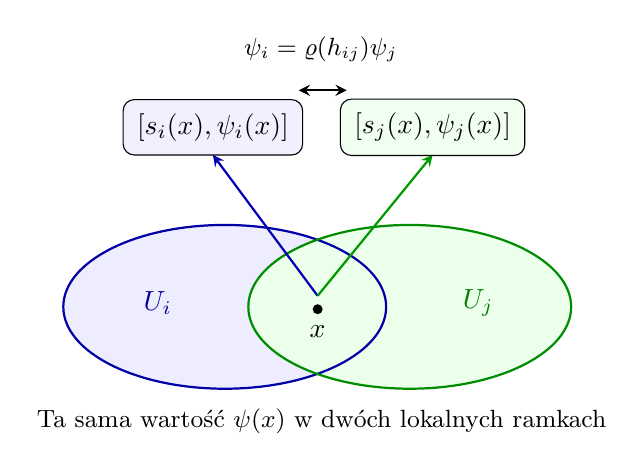
\begin{tikzpicture}[>=stealth,scale=1]
 \fill[blue!7] (-4.7,-1.1) ellipse (2.05 and 1.04);
 \fill[green!8] (-2.35,-1.1) ellipse (2.05 and 1.04);
 \draw[blue!65!black,thick] (-4.7,-1.1) ellipse (2.05 and 1.04);
 \draw[green!55!black,thick] (-2.35,-1.1) ellipse (2.05 and 1.04);
 \fill[black] (-3.52,-1.13) circle (1.8pt);
 \node[below] at (-3.52,-1.22) {$x$};
 \node[blue!60!black] at (-5.55,-1.05) {$U_i$};
 \node[green!50!black] at (-1.48,-1.05) {$U_j$};
 \draw[->,thick,blue!70!black] (-3.52,-.96)--(-4.85,.83);
 \draw[->,thick,green!60!black] (-3.52,-.96)--(-2.06,.83);
 \node[draw,rounded corners,fill=blue!6,align=center,inner sep=5pt]
  at (-4.85,1.18) {$[s_i(x),\psi_i(x)]$};
 \node[draw,rounded corners,fill=green!6,align=center,inner sep=5pt]
  at (-2.06,1.18) {$[s_j(x),\psi_j(x)]$};
 \draw[<->,thick] (-3.76,1.65)--(-3.15,1.65);
 \node[font=\small] at (-3.48,2.17)
  {$\psi_i=\varrho(h_{ij})\psi_j$};
 \node[font=\small] at (-3.47,-2.55)
  {Ta sama wartość $\psi(x)$ w dwóch lokalnych ramkach};
\end{tikzpicture}

{\small\itshape Dwie lokalne reprezentacje jednego pola spinorowego.
Warunek sklejania zapewnia zgodność na przecięciu obszarów.}
\end{center}

Różniczkowanie pól spinorowych wymaga dodatkowego
wyboru koneksji na $S(M)$. Jej konstrukcja przez
koneksję Levi-Civity oraz lokalne prawa transformacji
należą do geometrii różniczkowej; tutaj ograniczamy się
do algebraicznej i wiązkowej struktury spinorów.


\par\smallskip
{\footnotesize\noindent\emph{Dalsza lektura:}
Rachunki z konwencją $v^2=-\|v\|^2$
można porównać z notatkami Briana Conrada,
\emph{Clifford algebras and spin groups},
\url{https://math.stanford.edu/~conrad/210CPage/handouts/clifford.pdf}.
Budowę struktur spinowych i opis przeszkody
$w_2$ rozwijają notatki Konstantina Wernliego,
\emph{Lecture Notes on Spin Geometry},
\url{https://arxiv.org/pdf/1911.09766}.
Obie lektury używają miejscami innej kolejności tematów.
Powyższy test znaków został dowiedziony bez użycia kohomologii;
jego interpretacja jako klasy w $H^2$ korzysta z teorii
kohomologii Čech, której tutaj nie dowodziliśmy.\par}
\clearpage
